% 若编译失败,且生成 .synctex(busy) 辅助文件,可能有两个原因:
% 1. 需要插入的图片不存在:Ctrl + F 搜索 'figure' 将这些代码注释/删除掉即可
% 2. 路径/文件名含中文或空格:更改路径/文件名即可

% ------------------------------------------------------------- %
% >> ------------------ 文章宏包及相关设置 ------------------ << %
% 设定文章类型与编码格式
    \documentclass[UTF8]{report}		

% 本文特殊宏包
    \usepackage{siunitx} % 埃米单位

% 本文的特殊宏定义
\def\Im{\mathrm{\,Im\,}}
\def\Re{\mathrm{\,Re\,}}
\def\Ln{\mathrm{\,Ln\,}}
\def\Arg{\mathrm{\,Arg\,}}
\def\Arccos{\mathrm{\,Arccos\,}}
\def\Arcsin{\mathrm{\,Arcsin\,}}
\def\Arctan{\mathrm{\,Arctan\,}}

% 通用宏定义
\def\N{\mathbb{N}}
\def\F{\mathbb{F}}
\def\Z{\mathbb{Z}}
\def\Q{\mathbb{Q}}
\def\R{\mathbb{R}}
\def\C{\mathbb{C}}
\def\T{\mathbb{T}}
\def\S{\mathbb{S}}
\def\A{\mathbb{A}}
\def\I{\mathscr{I}}
\def\d{\mathrm{d}}
\def\p{\partial}


% 导入基本宏包
    \usepackage[UTF8]{ctex}     % 设置文档为中文语言
    \usepackage{hyperref}  % 宏包:自动生成超链接 (此宏包与标题中的数学环境冲突)
    \hypersetup{
        colorlinks=true,    % false:边框链接 ; true:彩色链接
        citecolor={red},    % 文献引用颜色
        linkcolor={blue},   % 目录,公式,图表,脚注等内部链接颜色
        urlcolor={cyan},    % 网页 URL 链接颜色,包括 \href 中的 text
        % cyan 浅蓝色 
        % magenta 洋红色
        % yellow 黄色
        % black 黑色
        % white 白色
        % red 红色
        % green 绿色
        % blue 蓝色
        % gray 灰色
        % darkgray 深灰色
        % lightgray 浅灰色
        % brown 棕色
        % lime 石灰色
        % olive 橄榄色
        % orange 橙色
        % pink 粉红色
        % purple 紫色
        % teal 蓝绿色
        % violet 紫罗兰色
    }
    % \usepackage{docmute}    % 宏包:子文件导入时自动去除导言区,用于主/子文件的写作方式,\include{./51单片机笔记}即可。注:启用此宏包会导致.tex文件capacity受限。
    \usepackage{amsmath}    % 宏包:数学公式
    \usepackage{mathrsfs}   % 宏包:提供更多数学符号
    \usepackage{amssymb}    % 宏包:提供更多数学符号
    \usepackage{pifont}     % 宏包:提供了特殊符号和字体
    \usepackage{extarrows}  % 宏包:更多箭头符号
    \usepackage{multicol}   % 宏包:支持多栏 


% 文章页面margin设置
    \usepackage[a4paper]{geometry}
        \geometry{top=1in}  % 1 inch= 2.46 cm, 0.75 inch = 1.85 cm
        \geometry{bottom=1in}
        \geometry{left=0.75in}
        \geometry{right=0.75in}   % 设置上下左右页边距
        \geometry{marginparwidth=1.75cm}    % 设置边注距离(注释、标记等)

% 配置数学环境
    \usepackage{amsthm} % 宏包:数学环境配置
    % theorem-line 环境自定义
        \newtheoremstyle{MyLineTheoremStyle}% <name>
            {11pt}% <space above>
            {11pt}% <space below>
            {\kaishu}% <body font> 使用默认正文字体
            {}% <indent amount>
            {\bfseries}% <theorem head font> 设置标题项为加粗
            {:}% <punctuation after theorem head>
            {.5em}% <space after theorem head>
            {\textbf{#1}\thmnumber{#2}\ \ (\,\textbf{#3}\,)}% 设置标题内容顺序
        \theoremstyle{MyLineTheoremStyle} % 应用自定义的定理样式
        \newtheorem{LineTheorem}{Theorem.\,}
    % theorem-block 环境自定义
        \newtheoremstyle{MyBlockTheoremStyle}% <name>
            {11pt}% <space above>
            {11pt}% <space below>
            {}% <body font> 使用默认正文字体
            {}% <indent amount>
            {\bfseries}% <theorem head font> 设置标题项为加粗
            {:\\ \indent}% <punctuation after theorem head>
            {.5em}% <space after theorem head>
            {\textbf{#1}\thmnumber{#2}\ \ (\,\textbf{#3}\,)}% 设置标题内容顺序
        \theoremstyle{MyBlockTheoremStyle} % 应用自定义的定理样式
        \newtheorem{BlockTheorem}[LineTheorem]{Theorem.\,} % 使用 LineTheorem 的计数器
    % definition 环境自定义
        \newtheoremstyle{MySubsubsectionStyle}% <name>
            {11pt}% <space above>
            {11pt}% <space below>
            {}% <body font> 使用默认正文字体
            {}% <indent amount>
            {\bfseries}% <theorem head font> 设置标题项为加粗
            {:\\ \indent}% <punctuation after theorem head>
            {0pt}% <space after theorem head>
            {\textbf{#3}}% 设置标题内容顺序
        \theoremstyle{MySubsubsectionStyle} % 应用自定义的定理样式
        \newtheorem{definition}{}

%宏包:有色文本框(proof环境)及其设置
    \usepackage[dvipsnames,svgnames]{xcolor}    %设置插入的文本框颜色
    \usepackage[strict]{changepage}     % 提供一个 adjustwidth 环境
    \usepackage{framed}     % 实现方框效果
        \definecolor{graybox_color}{rgb}{0.95,0.95,0.96} % 文本框颜色。修改此行中的 rgb 数值即可改变方框纹颜色,具体颜色的rgb数值可以在网站https://colordrop.io/ 中获得。(截止目前的尝试还没有成功过,感觉单位不一样)(找到喜欢的颜色,点击下方的小眼睛,找到rgb值,复制修改即可)
        \newenvironment{graybox}{%
        \def\FrameCommand{%
        \hspace{1pt}%
        {\color{gray}\small \vrule width 2pt}%
        {\color{graybox_color}\vrule width 4pt}%
        \colorbox{graybox_color}%
        }%
        \MakeFramed{\advance\hsize-\width\FrameRestore}%
        \noindent\hspace{-4.55pt}% disable indenting first paragraph
        \begin{adjustwidth}{}{7pt}%
        \vspace{2pt}\vspace{2pt}%
        }
        {%
        \vspace{2pt}\end{adjustwidth}\endMakeFramed%
        }

% 外源代码插入设置
    % matlab 代码插入设置
    \usepackage{matlab-prettifier}
        \lstset{style=Matlab-editor}    % 继承 matlab 代码高亮 , 此行不能删去
    \usepackage[most]{tcolorbox} % 引入tcolorbox包 
    \usepackage{listings} % 引入listings包
        \tcbuselibrary{listings, skins, breakable}
        \newfontfamily\codefont{Consolas} % 定义需要的 codefont 字体
        \lstdefinestyle{MatlabStyle_inc}{   % 插入代码的样式
            language=Matlab,
            basicstyle=\small\ttfamily\codefont,    % ttfamily 确保等宽 
            breakatwhitespace=false,
            breaklines=true,
            captionpos=b,
            keepspaces=true,
            numbers=left,
            numbersep=15pt,
            showspaces=false,
            showstringspaces=false,
            showtabs=false,
            tabsize=2,
            xleftmargin=15pt,   % 左边距
            %frame=single, % single 为包围式单线框
            frame=shadowbox,    % shadowbox 为带阴影包围式单线框效果
            %escapeinside=``,   % 允许在代码块中使用 LaTeX 命令 (此行无用)
            %frameround=tttt,    % tttt 表示四个角都是圆角
            framextopmargin=0pt,    % 边框上边距
            framexbottommargin=0pt, % 边框下边距
            framexleftmargin=5pt,   % 边框左边距
            framexrightmargin=5pt,  % 边框右边距
            rulesepcolor=\color{red!20!green!20!blue!20}, % 阴影框颜色设置
            %backgroundcolor=\color{blue!10}, % 背景颜色
        }
        \lstdefinestyle{MatlabStyle_src}{   % 插入代码的样式
            language=Matlab,
            basicstyle=\small\ttfamily\codefont,    % ttfamily 确保等宽 
            breakatwhitespace=false,
            breaklines=true,
            captionpos=b,
            keepspaces=true,
            numbers=left,
            numbersep=15pt,
            showspaces=false,
            showstringspaces=false,
            showtabs=false,
            tabsize=2,
        }
        \newtcblisting{matlablisting}{
            %arc=2pt,        % 圆角半径
            % 调整代码在 listing 中的位置以和引入文件时的格式相同
            top=0pt,
            bottom=0pt,
            left=-5pt,
            right=-5pt,
            listing only,   % 此句不能删去
            listing style=MatlabStyle_src,
            breakable,
            colback=white,   % 选一个合适的颜色
            colframe=black!0,   % 感叹号后跟不透明度 (为 0 时完全透明)
        }
        \lstset{
            style=MatlabStyle_inc,
        }
% table 支持
    \usepackage{booktabs}   % 宏包:三线表
    \usepackage{tabularray} % 宏包:表格排版
    \usepackage{longtable}  % 宏包:长表格

% figure 设置
    \usepackage{graphicx}  % 支持 jpg, png, eps, pdf 图片 
    \usepackage{svg}       % 支持 svg 图片
        \svgsetup{
            % 指向 inkscape.exe 的路径
            %inkscapeexe = C:/aa_MySame/inkscape/bin/inkscape.exe, 
            inkscapeexe = C:/aa_MySame/inkscape/bin/inkscape.exe, 
            % 一定程度上修复导入后图片文字溢出几何图形的问题
            inkscapelatex = false                 
        }
    \usepackage{subcaption} % subfigure 子图支持

% 图表进阶设置
    \usepackage{caption}    % 图注、表注
        \captionsetup[figure]{name=图}  
        \captionsetup[table]{name=表}
        \captionsetup{labelfont=bf, font=small}
    \usepackage{float}     % 图表位置浮动设置 

% 圆圈序号自定义
    \newcommand*\circled[1]{\tikz[baseline=(char.base)]{\node[shape=circle,draw,inner sep=0.8pt, line width = 0.03em] (char) {\small \bfseries #1};}}   % TikZ solution

% 列表设置
    \usepackage{enumitem}   % 宏包:列表环境设置
        \setlist[enumerate]{
            label=\bfseries(\arabic*) ,   % 设置序号样式为加粗的 (1) (2) (3)
            ref=\arabic*, % 如果需要引用列表项,这将决定引用格式(这里仍然使用数字)
            itemsep=0pt, parsep=0pt, topsep=0pt, partopsep=0pt, leftmargin=3.5em} 
        \setlist[itemize]{itemsep=0pt, parsep=0pt, topsep=0pt, partopsep=0pt, leftmargin=3.5em}
        \newlist{circledenum}{enumerate}{1} % 创建一个新的枚举环境  
        \setlist[circledenum,1]{  
            label=\protect\circled{\arabic*}, % 使用 \arabic* 来获取当前枚举计数器的值,并用 \circled 包装它  
            ref=\arabic*, % 如果需要引用列表项,这将决定引用格式(这里仍然使用数字)
            itemsep=0pt, parsep=0pt, topsep=0pt, partopsep=0pt, leftmargin=3.5em
        }  

% 其它设置
    % 脚注设置
        \renewcommand\thefootnote{\ding{\numexpr171+\value{footnote}}}
    % 参考文献引用设置
        \bibliographystyle{unsrt}   % 设置参考文献引用格式为unsrt
        \newcommand{\upcite}[1]{\textsuperscript{\cite{#1}}}     % 自定义上角标式引用
    % 文章序言设置
        \newcommand{\cnabstractname}{序言}
        \newenvironment{cnabstract}{%
            \par\Large
            \noindent\mbox{}\hfill{\bfseries \cnabstractname}\hfill\mbox{}\par
            \vskip 2.5ex
            }{\par\vskip 2.5ex}

% 文章默认字体设置
    \usepackage{fontspec}   % 宏包:字体设置
        \setmainfont{SimSun}    % 设置中文字体为宋体字体
        \setCJKmainfont[AutoFakeBold=3]{SimSun} % 设置加粗字体为 SimSun 族,AutoFakeBold 可以调整字体粗细
        \setmainfont{Times New Roman} % 设置英文字体为Times New Roman

% 各级标题自定义设置
    \usepackage{titlesec}   
        \titleformat{\chapter}[hang]{\normalfont\huge\bfseries\centering}{第\,\thechapter\,章}{20pt}{}
        \titlespacing*{\chapter}{0pt}{-20pt}{20pt} % 控制上方空白的大小
        % section标题自定义设置 
        \titleformat{\section}[hang]{\normalfont\Large\bfseries}{§\,\thesection\,}{8pt}{}
        % subsubsection标题自定义设置
        %\titleformat{\subsubsection}[hang]{\normalfont\bfseries}{}{8pt}{}

% >> ------------------ 文章宏包及相关设置 ------------------ << %
% ------------------------------------------------------------- %

% ----------------------------------------------------------- %
% >> --------------------- 文章信息区 --------------------- << %
% 页眉页脚设置
    \usepackage{fancyhdr}   %宏包:页眉页脚设置
        \pagestyle{fancy}
        \fancyhf{}
        \cfoot{\thepage}
        \renewcommand\headrulewidth{1pt}
        \renewcommand\footrulewidth{0pt}
        \lhead{2024.8 -- 2025.1} 
        \chead{here is the header,这里是页眉}    
        \rhead{dingyi233@mails.ucas.ac.cn}
%文档信息设置
    \title{这里是标题\\The Title of the Report}
    \author{丁毅\\ \footnotesize 中国科学院大学,北京 100049\\ Yi Ding \\ \footnotesize University of Chinese Academy of Sciences, Beijing 100049, China}
    \date{\footnotesize 2024.8 -- 2025.1}
% >> --------------------- 文章信息区 --------------------- << %
% ----------------------------------------------------------- %

% 开始编辑文章

\begin{document} 
\zihao{5}             % 设置全文字号大小, -4 为小四, 5 为五号

% --------------------------------------------------------------- %
% >> --------------------- 封面序言与目录 --------------------- << %
% 封面
    \maketitle\newpage  
    \pagenumbering{Roman} % 页码为大写罗马数字
    \thispagestyle{fancy}   % 显示页码、页眉等

% 序言
\begin{cnabstract}\normalsize 
    本文为笔者本科时的“某某”课程笔记(Notes of balabala, 2024.9 -- 2025.1)。课程信息、作业与相关资料可以在笔者的个人网站上找到: \href{https://yidingg.github.io/YiDingg}{Notes > 这里给网址导航 (https://yidingg.github.io/YiDingg)},参考文献会在课程结束后统一上传到网址 {\color{red}(待更新)}。
    
    由于个人学识浅陋,认识有限,文中难免有不妥甚至错误之处,望读者不吝指正。可以将错误发送到我的邮箱 {\color{cyan}\ dingyi233@mails.ucas.ac.cn},也可以到笔者的 \href{https://github.com/YiDingg/LatexNotes}{GitHub 笔记库 (https://github.com/YiDingg/LatexNotes)} 提 issue,衷心感谢。
\end{cnabstract}
\addcontentsline{toc}{chapter}{序言} % 手动添加为目录

% 目录
    \setcounter{tocdepth}{2}                % 目录深度(为1时显示到section)
    \tableofcontents                        % 目录页
    \addcontentsline{toc}{chapter}{目录}    % 手动添加此页为目录
    \thispagestyle{fancy}                   % 显示页码、页眉等 

% 收尾工作
    \newpage    
    \pagenumbering{arabic} 


% >> --------------------- 封面序言与目录 --------------------- << %
% --------------------------------------------------------------- %


\chapter{基础知识}\thispagestyle{fancy} 
\section{第一章第一节}


\begin{definition}[向后加权隐式格式]

将向前差分与向后差分加权组合起来,得到:

\begin{equation}\label{公式5}
    \frac{u_{j}^{k}-u_{j}^{k-1}}{h_t}=a\theta\frac{u_{j+1}^{k}-2u_{j}^{k}+u_{j-1}^{k}}{h_x^2}+a(1-\theta)\frac{u_{j+1}^{k-1}-2u_{j}^{k-1}+u_{j-1}^{k-1}}{h_x^2}
\end{equation}

其中 $\theta \in [0, 1]$ 为权重,其截断误差 $R = a\left(\frac{1}{2}-\theta\right)h_t\left[\frac{\partial^{3}u}{\partial x^{2}\partial t}\right]_{j}^{k}+O(h_t^{2}+h_x^2)$,因此当 $\theta = \frac{1}{2}$ 时,方程具有 $O(h_t^{2}+h_x^2)$ 精度,称为 Crank-Nicolson 格式(CN 格式)。


公式 \ref{公式5} 的增长因子及稳定性条件为:

\begin{equation}
    G(h_t,\sigma)=\frac{1-4(1-\theta)ar\sin^2\frac{\sigma h}2}{1+4\theta ar\sin^2\frac{\sigma h}2}, \ \ 
    \begin{cases}
        r\leqslant\frac{1}{2a(1-2\theta)}, & \theta \in [0, \frac{1}{2}) \\ 
        \text{无条件稳定}, & \theta \in [\frac{1}{2}, 1] \\ 
    \end{cases}
\end{equation}


\begin{LineTheorem}[这是一个 Line Theorem]\label{这是一个 Line Theorem}
    你好你好你好
\end{LineTheorem}

\begin{BlockTheorem}[这是一个 Block Theorem]\label{这是一个 Block Theorem}
    你好你好你好
\end{BlockTheorem}



\begin{graybox}
\textbf{定理 \ref{这是一个 Block Theorem} 的证明:}\\
你好你好你好
\end{graybox}

\begin{figure}[H]
    \centering
    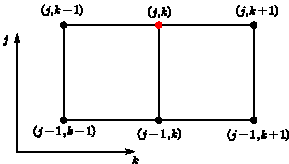
\includegraphics[width=0.5\textwidth]{assets/差分格式示意图.pdf}
    \caption{\textbf{插入pdf图片}}\label{插入pdf图片}
\end{figure}

\begin{figure}[H]
    \centering
    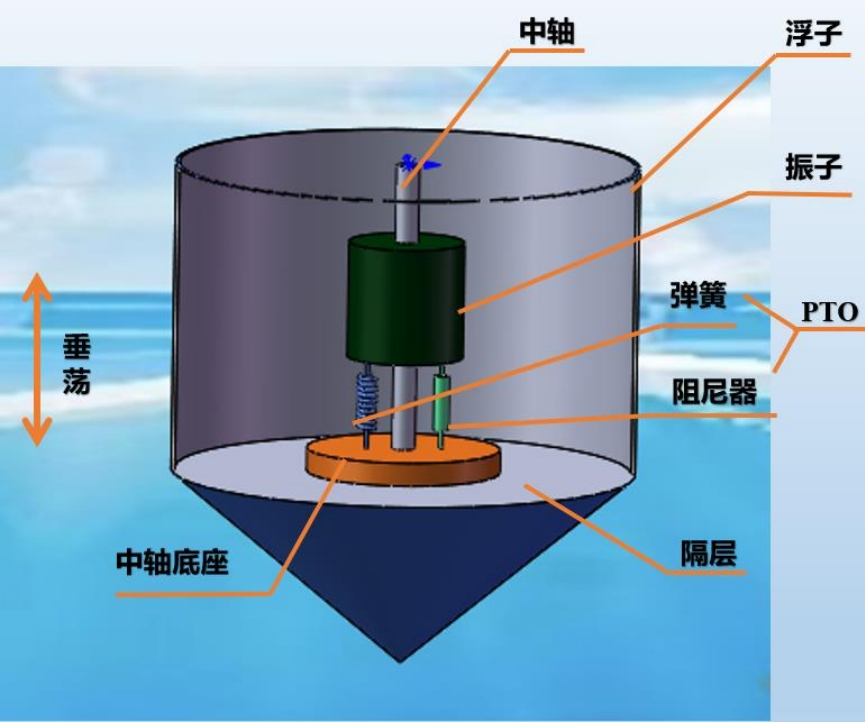
\includegraphics[width=0.5\textwidth]{assets/波浪能装置示意图.jpg}
    \caption{\textbf{插入 jpg}}\label{插入 jpg}
\end{figure}

\begin{figure}[H]
    \centering
    \includesvg[width=0.5\textwidth]{assets/draw.io_test.drawio.svg}
    \caption{\textbf{插入 svg}}\label{插入 svg}
\end{figure}

\end{definition}

表格:

\begin{table}[H]
    \centering
    \caption{\textbf{符号含义与约定}}
    \label{tab:waterpump}
    \begin{tabular}{ccccc}
    \toprule
    符号 & 符号含义& 单位\\
    \midrule
    符号1& 含义1& 单位1\\
    符号2& 含义2& 单位2\\
    符号3& 含义3& 单位3\\
    符号4& 含义4& 单位4\\
    \bottomrule
    \end{tabular}
\end{table}

\chapter{这里是第二章}\thispagestyle{fancy} 













% ----------------------------------------------------------- %
% >> ---------------------- 参考文献 ---------------------- << %
\nocite{*}
\bibliography{re}
\thispagestyle{fancy} 
\addcontentsline{toc}{chapter}{参考文献}
% >> ---------------------- 参考文献 ---------------------- << %
% ----------------------------------------------------------- %
















% ------------------------------------------------------------ %
% >> ------------------------ 附录 ------------------------ << %

% 附录设置
\newpage
\appendix
% chapter 标题自定义设置
\titleformat{\chapter}[hang]{\normalfont\huge\bfseries\centering}{}{20pt}{}
\titlespacing*{\chapter}{0pt}{-25pt}{8pt} % 控制上方空白的大小
% section 标题自定义设置 
\titleformat{\section}[hang]{\normalfont\centering\Large\bfseries}{\thesection}{8pt}{}

% 附录 A
\chapter*{附录 A\hspace*{20pt}  某某课程 Q \& A}\setcounter{chapter}{1} 
\setcounter{equation}{0}    % 重置公式计数器   
\addcontentsline{toc}{chapter}{附录 A\hspace*{6pt}  某某课程 Q \& A}   
\thispagestyle{fancy} 
\setcounter{section}{0}   
\renewcommand\thesection{A.\arabic{section}}   
\renewcommand{\thefigure}{A.\arabic{figure}} 
\renewcommand{\thetable}{A.\arabic{table}}

\section{第一章}
\section{第二章}

% 附录 B
\chapter*{附录 B\hspace*{20pt}  中英文对照表}
\setcounter{chapter}{2} 
\setcounter{equation}{0}    % 重置公式计数器   
\addcontentsline{toc}{chapter}{附录 B\hspace*{6pt}  中英文对照表}   
\thispagestyle{fancy} 
\setcounter{section}{0}   
\renewcommand\thesection{B.\arabic{section}}   
\renewcommand{\thefigure}{B.\arabic{figure}} 
\renewcommand{\thetable}{B.\arabic{table}}

\section{中英文对照表}
\begin{multicols}{2}  

    \begin{table}[H]\centering
    \caption{\textbf{中英文对照表}}
    \begin{tabular}{cccccccc}\toprule
        English & 中文 \\
        \midrule
        voltage            & 电压 \\
        current            & 电流 \\
        power              & 功率 \\
        resistance         & 电阻 \\
        conductance        & 电导 \\
        inductance         & 电感 \\
        capacitance        & 电容 \\
        frequency          & 频率 \\
        circuit            & 电路 \\
        circuit element    & 电流元件 \\
        signal             & 信号 \\
        circuit analysis   & 电路分析 \\
        circuit synthesis  & 电路综合 \\
        circuit design     & 电路设计 \\
        circuit topology   & 电路拓扑 \\
        \bottomrule
    \end{tabular}
    \end{table}
    
    \begin{table}[H]\centering
        \caption{\textbf{中英文对照表}}
        \begin{tabular}{cccccccc}\toprule
            English & 中文 \\
            \midrule
            voltage            & 电压 \\
            current            & 电流 \\
            power              & 功率 \\
            resistance         & 电阻 \\
            conductance        & 电导 \\
            inductance         & 电感 \\
            capacitance        & 电容 \\
            frequency          & 频率 \\
            circuit            & 电路 \\
            circuit element    & 电流元件 \\
            signal             & 信号 \\
            circuit analysis   & 电路分析 \\
            circuit synthesis  & 电路综合 \\
            circuit design     & 电路设计 \\
            circuit topology   & 电路拓扑 \\
            \bottomrule
        \end{tabular}
    \end{table}
\end{multicols} 


% 附录 C
\chapter*{附录 C\hspace*{20pt} Matlab 源代码}\addcontentsline{toc}{chapter}{附录 C\hspace*{6pt}  Matlab 源代码}   
\thispagestyle{fancy} 
\setcounter{section}{0}   
\renewcommand\thesection{C.\arabic{section}}   
\renewcommand{\thefigure}{C.\arabic{figure}} 
\renewcommand{\thetable}{C.\arabic{table}}

% 注意:listing环境中手动输入的代码需要顶格写

\begin{matlablisting}
% MATLAB code here
x = 0:0.1:2*pi;
y = sin(x);
plot(x, y);
xlabel('x');
ylabel('sin(x)');
title('Sine Function');
% ... (MATLAB code here,最好是插入文件)
% MATLAB code here
x = 0:0.1:2*pi;
y = sin(x);
plot(x, y);
xlabel('x');
ylabel('sin(x)');
title('Sine Function');
% ... (MATLAB code here,最好是插入文件)
% MATLAB code here
x = 0:0.1:2*pi;
y = sin(x);
plot(x, y);
xlabel('x');
ylabel('sin(x)');
title('Sine Function');
% ... (MATLAB code here,最好是插入文件)
% MATLAB code here
x = 0:0.1:2*pi;
y = sin(x);
plot(x, y);
xlabel('x');
ylabel('sin(x)');
title('Sine Function');
% ... (MATLAB code here,最好是插入文件)
% MATLAB code here
x = 0:0.1:2*pi;
y = sin(x);
plot(x, y);
xlabel('x');
ylabel('sin(x)');
title('Sine Function');
% ... (MATLAB code here,最好是插入文件)
% MATLAB code here
x = 0:0.1:2*pi;
y = sin(x);
plot(x, y);
xlabel('x');
ylabel('sin(x)');
title('Sine Function');
% ... (MATLAB code here,最好是插入文件)% ... (MATLAB code here,最好是插入文件)% ... (MATLAB code here,最好是插入文件)% ... (MATLAB code here,最好是插入文件)% ... (MATLAB code here,最好是插入文件)A
% MATLAB code here
x = 0:0.1:2*pi;
y = sin(x);
plot(x, y);
xlabel('x');
ylabel('sin(x)');
title('Sine Function');
% ... (MATLAB code here,最好是插入文件)
\end{matlablisting}

% >> ------------------------ 附录 ------------------------ << %
% ------------------------------------------------------------ %

\end{document}



% VScode 常用快捷键:

% F2:                       变量重命名
% Ctrl + Enter:             行中换行
% Alt + up/down:            上下移行
% 鼠标中键 + 移动:           快速多光标
% Shift + Alt + up/down:    上下复制
% Ctrl + left/right:        左右跳单词
% Ctrl + Backspace/Delete:  左右删单词    
% Shift + Delete:           删除此行
% Ctrl + J:                 打开 VScode 下栏(输出栏)
% Ctrl + B:                 打开 VScode 左栏(目录栏)
% Ctrl + `:                 打开 VScode 终端栏
% Ctrl + 0:                 定位文件
% Ctrl + Tab:               切换已打开的文件(切标签)
% Ctrl + Shift + P:         打开全局命令(设置)

% Latex 常用快捷键

% Ctrl + Alt + J:           由代码定位到PDF
% 


% Git提交规范:
% update: Linear Algebra 2 notes
% add: Linear Algebra 2 notes
% import: Linear Algebra 2 notes
% delete: Linear Algebra 2 notes

